% This file was created by tikzplotlib v0.9.2.
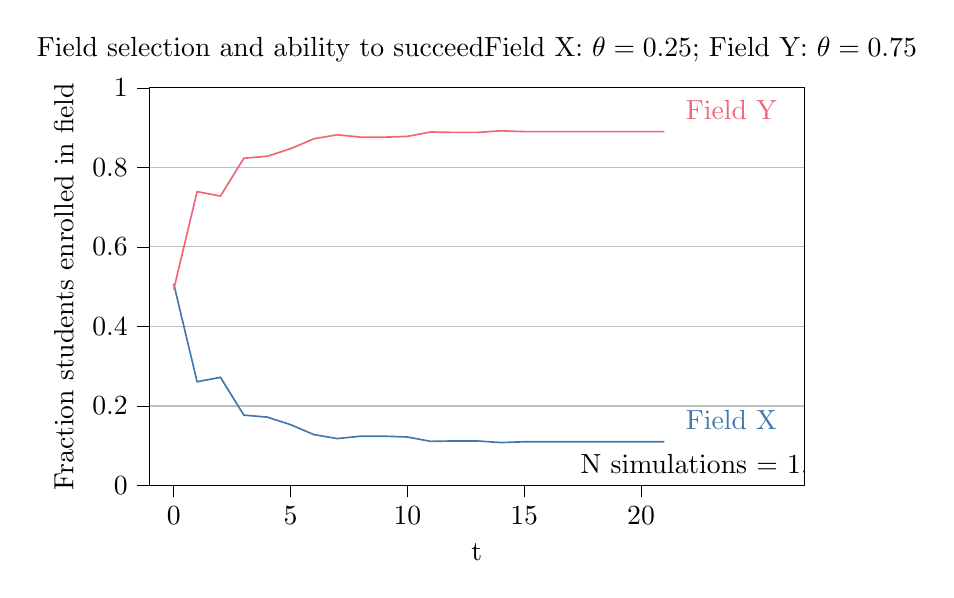
\begin{tikzpicture}

\definecolor{color0}{rgb}{0.266666666666667,0.466666666666667,0.666666666666667}
\definecolor{color1}{rgb}{0.933333333333333,0.4,0.466666666666667}

\begin{axis}[
height=6.6314113761540705cm,
tick align=outside,
tick pos=left,
title={Field selection and ability to succeed \\ Field X: \(\displaystyle \theta = 0.25\); Field Y: \(\displaystyle \theta = 0.75\)},
width=9.904475999999999cm,
x grid style={white!69.0196078431373!black},
xlabel={t},
xmin=-1.05, xmax=27,
xtick style={color=black},
xtick={0,5,10,15,20},
xticklabels={\(\displaystyle 0\),\(\displaystyle 5\),\(\displaystyle 10\),\(\displaystyle 15\),\(\displaystyle 20\)},
ylabel={Fraction students enrolled in field},
ymajorgrids,
ymin=0, ymax=1,
ytick style={color=black},
ytick={0,0.2,0.4,0.6,0.8,1},
yticklabels={\(\displaystyle 0\),\(\displaystyle 0.2\),\(\displaystyle 0.4\),\(\displaystyle 0.6\),\(\displaystyle 0.8\),\(\displaystyle 1\)}
]
\addplot [semithick, color0]
table {%
0 0.506999969482422
1 0.261000037193298
2 0.272000074386597
3 0.177000045776367
4 0.172000050544739
5 0.152999997138977
6 0.128000020980835
7 0.118000030517578
8 0.123999953269958
9 0.123999953269958
10 0.121999979019165
11 0.111000061035156
12 0.111999988555908
13 0.111999988555908
14 0.108000040054321
15 0.110000014305115
21 0.110000014305115
};
\addplot [semithick, color1]
table {%
0 0.493000030517578
1 0.739000082015991
2 0.727999925613403
3 0.822999954223633
4 0.828000068664551
5 0.847000002861023
6 0.871999979019165
7 0.881999969482422
8 0.875999927520752
9 0.875999927520752
10 0.878000020980835
11 0.888999938964844
12 0.888000011444092
13 0.888000011444092
14 0.891999959945679
15 0.889999985694885
21 0.889999985694885
};
\draw (axis cs:21.5,0.14) node[
  anchor=base west,
  text=color0,
  rotate=0.0
]{Field X};
\draw (axis cs:21.5,0.92) node[
  anchor=base west,
  text=color1,
  rotate=0.0
]{Field Y};
\draw (axis cs:17,0.03) node[
  anchor=base west,
  text=black,
  rotate=0.0
]{N simulations = 1,000};
\end{axis}

\end{tikzpicture}
